
\chapter{مطالعات پیشین}

در این فصل، به مرور مطالعات پیشین و روش‌های مرتبط ترمیم تصویر پرداخته می‌شود. هدف از این مرور، شناسایی نقاط قوت و ضعف روش‌های موجود، بررسی پیشرفت‌های اخیر در حوزه مرتبط، بررسی مجموعه‌داده های ترمیم تصویر و ارائه پیش‌زمینه ای از متدولوژی های مرسوم ترمیم است.

ابتدا به بررسی تاریخچه و پیشرفت روش‌های مرتبط با ترمیم تصاویر پرداخته خواهد شد و دسته‌بندی‌های مختلف این روش‌ها، به همراه مزایا و معایب آن‌ها مورد بحث قرار خواهد گرفت. سپس، مجموعه داده‌های مورد استفاده در این حوزه معرفی شده و معیارهای مورد نظر برای ارزیابی این روش‌ها توضیح داده می‌شوند. در نهایت، الگوریتم‌های کلاسیک و روش‌های مبتنی بر یادگیری عمیق که تاکنون برای ترمیم تصاویر پیشنهاد شده‌اند، بررسی خواهند شد. این تحلیل به عنوان مبنایی برای توجیه ضرورت استفاده از معماری ترنسفورمر در تحقیق حاضر خواهد بود.

\section{روش های الگوریتمی}

مسئله ترمیم تصویر به قبل‌تر از ظهور روش‌های مبتنی بر یادگیری عمیق بازمی‌گردد. در ابتدا این مسئله به کمک روش‌های الگوریتمی کلاسیک مورد بررسی قرار گرفت. یکی از اولین روش‌های مطرح‌شده در حوزه ترمیم تصاویر، رویکرد مبتنی بر انتشار بود که توسط Bertalmio و همکارانش در سال ۲۰۰۰ معرفی شد \cite{bertalmioImageInpainting2000}. این روش از معادلات دیفرانسیل جزئی \lr{(PDE)} برای گسترش اطلاعات موجود در لبه‌های تصویر به نواحی آسیب‌دیده استفاده می‌کند. ایده اصلی این روش، شبیه‌سازی فرآیند طبیعی انتشار اطلاعات در تصویر است تا ساختارهای محلی به صورت پیوسته بازسازی شوند. با وجود اینکه این روش برای ترمیم نواحی کوچک و حفظ ساختار لبه‌ها عملکرد خوبی دارد، اما روشی ابتدایی مبتنی بر محلی ترین مفروضات تصویر بوده و در بازسازی نواحی بزرگ‌تر یا بافت‌های پیچیده به دلیل محدودیت درک محتوای کلی تصویر ناکارآمد است.

در ادامه رویکردهای مبتنی بر انتشار، روش ترمیم تصویر با تغییرات کل \lr{(Total Variation Inpainting)} که توسط Chan و Shen در سال ۲۰۰۱ معرفی شد \cite{chanNontextureInpaintingCurvatureDriven2001}، گامی دیگر در پیشرفت این حوزه بود. این روش بر مبنای به حداقل رساندن یک تابع انرژی طراحی شده است که هدف آن حفظ ساختار لبه‌ها و جلوگیری از ایجاد تاری در نواحی بازسازی‌شده است. مدل تغییرات کل از معادلات دیفرانسیل جزئی برای انتقال اطلاعات لبه‌ها به نواحی آسیب‌دیده استفاده می‌کند و توانایی بالایی در بازسازی ساختارهای ساده دارد. با این حال، مانند روش Bertalmio و همکاران، این رویکرد نیز در بازسازی بافت‌های پیچیده یا نواحی بزرگ با محدودیت‌هایی مواجه است.


دسته دیگری از روش‌های کلاسیک که به مراتب موفق تر عمل کردند، روش‌های مبتنی بر وصله \lr{(Patch-Based Methods)} بودند. در این روش‌ها، نواحی سالم تصویر به عنوان بانک وصله‌ها در نظر گرفته می‌شدند و بهترین تطابق برای پر کردن نواحی آسیب‌دیده از میان این وصله‌ها انتخاب می‌شد.

به‌عنوان مثال در یکی از برجسته ترین روش های غیرمبتنی بر یادگیری، بارنز و همکاران در \cite{barnesPatchMatchRandomizedCorrespondence2009} با معرفی PatchMatch ابزارهای تعاملی ویرایش تصویر را با استفاده از یک الگوریتم تصادفی جدید ارائه داده‌اند که امکان یافتن بسیار سریع تطابق‌های تقریبی نزدیک‌ترین همسایه بین قطعات تصویر را فراهم می‌کند. الگوریتم ارائه‌شده توسط آن‌ها بهبودهای قابل‌توجهی در عملکرد نسبت به روش‌های پیشین (۲۰ تا ۱۰۰ برابر سریع‌تر) ارائه می‌دهد و استفاده از آن را در ابزارهای تعاملی ممکن می‌سازد. بینش‌های کلیدی این الگوریتم شامل یافتن برخی تطابق‌های مناسب از طریق نمونه‌گیری تصادفی و استفاده از هم‌بستگی طبیعی در تصاویر برای انتشار سریع این تطابق‌ها به نواحی مجاور است.

با وجود این که این رویکردها توانستند نتایج بهتری نسبت به روش های مبتنی بر PDE در بازسازی جزئیات ارائه دهند، اما به دلیل تکیه بر ویژگی‌های محلی و وابستگی به مشابهت بافتی، در مواجهه با تصاویر پیچیده و متنوع محدودیت‌های زیادی داشتند و اکثرا مفروضات عمیقی در مورد تصاویر هدفشان داشتند. یکی از این مفروضات، فرض رنک پایین بودن تصاویر است. این فرض بر این ایده استوار است که داده‌های تصویری در بسیاری از کاربردها، به‌ویژه در تصاویر طبیعی، به صورت ذاتی دارای ساختار رنک پایین هستند. به این معنا که اطلاعات موجود در یک تصویر را می‌توان در یک فضای برداری با ابعاد بسیار کمتر نسبت به فضای اصلی بازنمایی کرد. روش‌های مبتنی بر این فرض، مانند تجزیه مقدار منفرد \lr{(SVD)}
\cite{yaghmaeeImprovingImageInpainting2020}
 و فشرده‌سازی رنک پایین، در بسیاری از مسائل پردازش تصویر نظیر ترمیم تصویر، کاهش نویز و فشرده‌سازی داده به کار گرفته شدند. با این حال، این الگوریتم‌های کلاسیک اغلب در شرایط پیچیده‌تر مانند تصاویر با ساختار غیرخطی، نواحی هدف ترمیم بسیار بزرگ، نواحی بافت‌های پیچیده، یا تصاویر آسیب‌دیده با نویز بالا عملکرد ضعیفی داشتند. این محدودیت‌ها ناشی از این واقعیت است که تصاویر واقعی معمولاً از روابط غیرخطی پیچیده و وابستگی‌های بلندمدت میان پیکسل‌ها پیروی می‌کنند که فرض رنک پایین قادر به مدل‌سازی آن‌ها نیست. علاوه بر این، این روش‌ها اغلب فرض می‌کنند که اطلاعات کلیدی تصویر به صورت یکنواخت توزیع شده است، در حالی که در واقعیت، اطلاعات تصاویر در نواحی مختلف دارای توزیع‌های بسیار متفاوتی است.
 
 همچنین در ترمیم تصاویر با نواحی هدف ماسک شده بسیار بزرگ، روش های مبتنی بر وصله نیازمند وصله هایی مشابه در تصویر بودند تا با استفاده از آن ها، نواحی مورد نظر را ترمیم کنند. فرض استوار این روش ها بر این بود که برای هر تصویر $I$ شامل وصله‌هایی مانند $x = \{x_1, x_2, \dots, x_n\}$ است که می‌توانند از طریق ترکیب یا تبدیل‌های خطی و غیرخطی، ویژگی‌های معنایی دقیقی را برای بازسازی نواحی گمشده تولید کنند. به بیان ریاضی، این فرضیه به این معناست که برای هر وصله گمشده $x_{\text{missing}}$، می‌توان یک ترکیب بهینه از وصله‌های موجود $x_{\text{observed}}$ پیدا کرد که به صورت زیر بازسازی را انجام دهد:
 
 $$
 x_{\text{missing}} \approx \sum_{i=1}^{n} w_i \cdot T_i(x_i)
 $$


با این حال، با افزایش اندازه ماسک، یا ماسک کردن نواحی با الگو های پیچیده اما یکتا مانند چهره ها، این فرضیه دیگر معتبر نیست. در چنین حالتی، نواحی گمشده به‌حدی بزرگ هستند که وصله‌های مشابه کافی در تصویر وجود ندارد، یا ترکیب آن‌ها نمی‌تواند ویژگی‌های معنایی دقیق و نوآورانه مورد نیاز را تولید کند. در نتیجه، روش‌های مبتنی بر وصله نیز، در مواجهه با ماسک‌های بزرگ، به‌دلیل عدم توانایی در تولید ویژگی‌های معنایی جدید، با محدودیت مواجه می‌شوند.

\section{روش‌های مبتنی بر یادگیری عمیق}

با ظهور یادگیری عمیق و توانایی آن در استخراج ویژگی‌های پیچیده از داده‌های تصویری و همچنین تولید ویژگی های نوین لازم برای انواع چالش‌برانگیزی از مسائل ترمیم، پژوهش‌ها در زمینه ترمیم تصاویر به سمت استفاده از مدل‌های مبتنی بر شبکه‌های عصبی سوق یافت. این روش‌ها با استفاده از مجموعه داده‌های بزرگ و متنوع، قادر به یادگیری الگوهای پیچیده و بازسازی دقیق‌تر نواحی آسیب‌دیده شدند. برخلاف روش‌های الگوریتمی که عمدتاً بر اصول ریاضی و آماری استوار بودند، روش‌های مبتنی بر یادگیری امکان درک مفاهیم سطح بالا و روابط سراسری در تصویر را فراهم کردند و موفق شدند ترمیم هایی با  ماسک های بزرگ‌تر انجام دهند، چرا که این امر گاها نیازمند ساخت ساختار های کاملا جدید در تصویر (مانند ساختار چهره، طبیعت و ...) بود. 

\section{مجموعه‌داده‌های ترمیم تصویر}

یکی از عوامل کلیدی در موفقیت مدل‌های یادگیری عمیق در پردازش تصویر، وجود مجموعه‌داده‌های بزرگ و متنوع است که امکان آموزش مدل‌ها در سناریوهای گوناگون را فراهم می‌سازد. مجموعه‌داده‌های مختلف برای کاربردهای خاص طراحی شده‌اند و هر یک ویژگی‌های منحصربه‌فردی دارند. در ادامه، به معرفی برخی از مجموعه‌داده‌های شناخته‌شده مانند \lr{CelebA-HQ}، \lr{Places}، و چندین مجموعه‌داده دیگر پرداخته می‌شود.


مجموعه‌داده \textbf{CelebA-HQ} یکی از معروف‌ترین مجموعه‌داده‌ها برای تحلیل چهره است. این مجموعه‌داده‌ی کلاس‌بندی نشده، شامل تصاویری با وضوح بالا از چهره انسان است که ویژگی‌هایی مانند موقعیت، حالت، رنگ پوست، زاویه و روشنایی های مختلف را پوشش می‌دهد. CelebA-HQ به‌طور گسترده در زمینه‌هایی مانند بازسازی تصویر، تغییر چهره، و شناسایی چهره استفاده شده است. ویژگی برجسته این مجموعه‌داده، کیفیت بالای تصاویر و پوشش گسترده از حالات و ویژگی‌های مختلف چهره است که آن را به انتخابی محبوب برای مدل‌های یادگیری عمیق تبدیل کرده است.

\begin{figure}
	\centering
	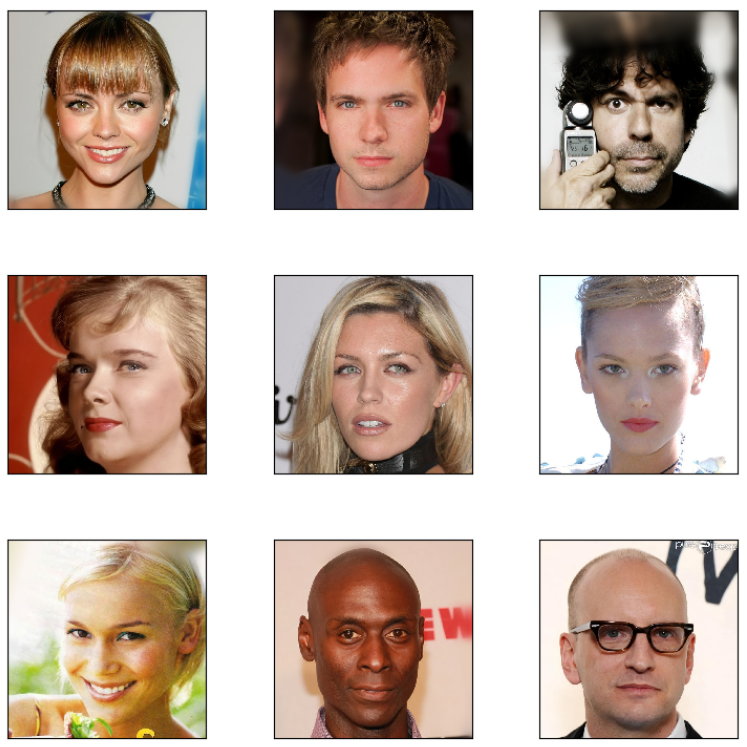
\includegraphics[width=0.7\linewidth]{celebahq1}
	\caption{نمونه تصاویر از مجموعه‌داده Celeb-A-HQ. تمرکز این دیتاست بر روی فیچر های چهره است.}
	\label{fig:celebahq1}
\end{figure}

مجموعه‌داده \textbf{Places} برای تحلیل صحنه‌ها و شناخت محیط‌ها طراحی شده است. این مجموعه‌داده‌ی کلاس‌بندی شده، شامل میلیون‌ها تصویر از محیط‌های مختلف مانند مناظر طبیعی، محیط‌های شهری، و فضاهای داخلی است. مجموعه Places برای کاربردهایی مانند تشخیص صحنه، طبقه‌بندی محیط، و تولید تصاویر صحنه استفاده می‌شود. یکی از ویژگی‌های کلیدی این مجموعه‌داده، تنوع بالا در دسته‌بندی‌های محیطی است که امکان آموزش مدل‌هایی با درک عمیق‌تر از صحنه‌های مختلف را فراهم می‌کند.

\begin{figure}
	\centering
	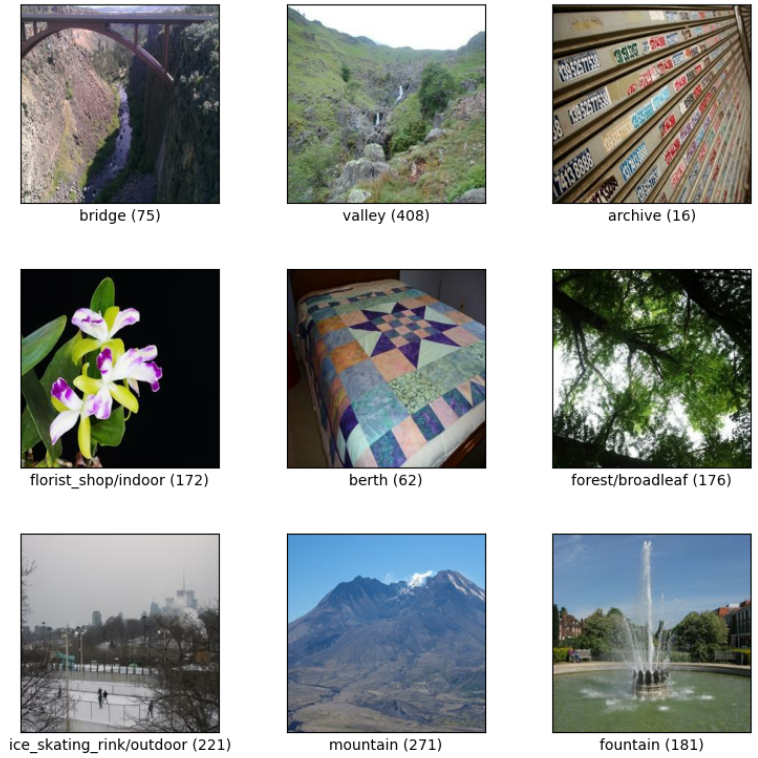
\includegraphics[width=0.7\linewidth]{places1}
	\caption{نمونه تصاویر از مجموعه‌داده Places به همراه یک کلمه برای توصیف هر تصویر و اندیس هر فایل در داخل پرانتز}
	\label{fig:places1}
\end{figure}


مجموعه‌داده \textbf{ImageNet} یکی از جامع‌ترین مجموعه‌داده‌های موجود در حوزه یادگیری عمیق است که با بیش از ۱۴ میلیون تصویر
\footnote{این مجموعه‌داده هر سال در حال بروزرسانی و افزوده شدن است. آمار ذکر شده آخرین آمار تا ژانویه ۲۰۲۵ است.}
در ۱۰۰۰ طبقه‌بندی مختلف تأثیر شگرفی بر پیشرفت شبکه‌های عصبی داشته است. ImageNet علاوه بر کاربردهای عمومی مانند طبقه‌بندی تصویر، به‌عنوان یک معیار استاندارد برای ارزیابی عملکرد مدل‌های یادگیری عمیق استفاده می‌شود. موفقیت‌های اولیه شبکه‌های عصبی کانولوشنی (CNN) مانند AlexNet و ResNet تا حد زیادی مرهون این مجموعه‌داده بزرگ و متنوع بوده‌اند.



%یکی دیگر از مجموعه‌داده‌های مهم، \textbf{MS-COCO} است که برای وظایف پیشرفته‌تری مانند تشخیص اشیا، بخش‌بندی تصویر، و توصیف تصویر طراحی شده است. این مجموعه‌داده شامل تصاویری است که حاوی چندین شیء از دسته‌بندی‌های مختلف هستند، و هر تصویر دارای برچسب‌های متنی دقیق و اطلاعات مربوط به موقعیت اشیاء است. MS-COCO به‌طور گسترده در مدل‌هایی که نیازمند درک پیچیده‌تر تصویر هستند، مانند مدل‌های تولید متن از تصویر
%\LTRfootnote{Image Captioning}
%یا سیستم‌های تشخیص چند‌شیء، استفاده می‌شود.
مجموعه داده
\lr{DTD (Describable Textures Dataset)}
یک مجموعه داده شامل $5640$ تصویر واقعی از بافت‌های مختلف است که با یک یا چند صفت توصیفی از یک واژگان ۴۷ کلمه‌ای در زبان انگلیسی برچسب‌گذاری شده‌اند. این مجموعه داده به‌طور خاص برای مطالعه و تحلیل بافت‌های قابل توصیف طراحی شده است و شامل نمونه‌هایی از بافت‌های طبیعی و مصنوعی است. 

از ویژگی‌های قابل توجه \lr{DTD} می‌توان به تنوع گسترده تصاویر و برچسب‌های توصیفی دقیق اشاره کرد که آن را به یک منبع ارزشمند در کاربردهایی نظیر دسته‌بندی بافت‌ها، تشخیص الگو و آموزش مدل‌های یادگیری عمیق تبدیل کرده است. این مجموعه داده برای ارزیابی مدل‌های بینایی کامپیوتر که نیاز به درک ویژگی‌های بصری بافت‌ها دارند، به‌ویژه در مسائل مرتبط با توصیف و دسته‌بندی، بسیار مناسب است.

در جدول \ref{tab:datasets_summary} خلاصه ای از مجموعه‌داده های بیان‌شده آورده شده است.
\warningToSelfExpandable

\begin{figure}
	\centering
	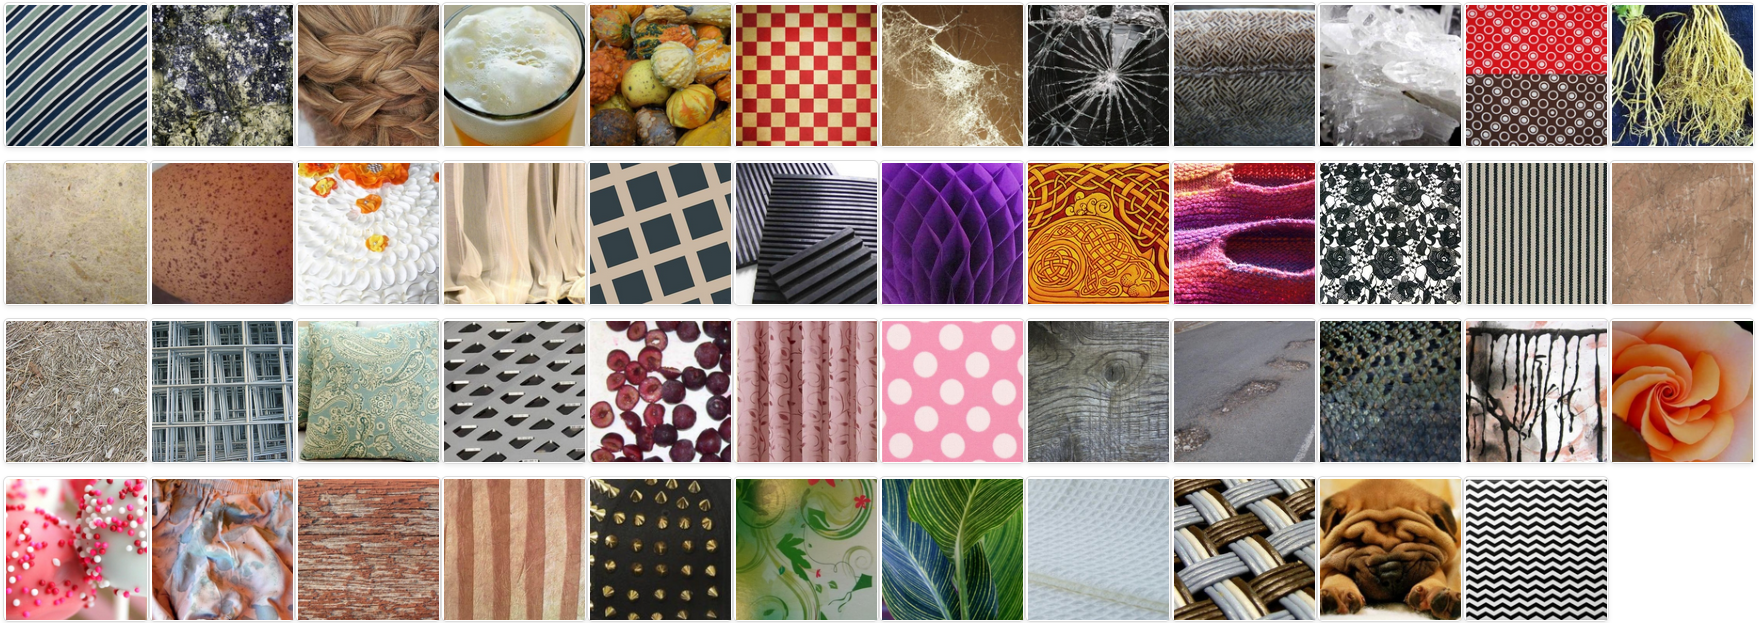
\includegraphics[width=0.7\linewidth]{dtd1}
	\caption{نمونه تصاویر مجموعه‌داده DTD}
	\label{fig:dtd1}
\end{figure}



\begin{table}
	\centering
	\label{tab:datasets_summary}
	\begin{tabular}{|l|c|c|l|}
		\hline
		\textbf{نام مجموعه داده} & \textbf{برچسب‌دار (بله/خیر)} & \textbf{تعداد تصاویر} & \textbf{ویژگی} \\ \hline
		\lr{Places2} \cite{zhouPlacesImageDatabase2016} & بله & $>10,000,000$ & محیط‌ها \\ \hline
		\lr{CelebA} \cite{liuDeepLearningFace2015} & بله & $200,000$ & چهره \\ \hline
		\lr{CelebHQ} \cite{karrasProgressiveGrowingGANs2018} & بله & $30,000$ & چهره با کیفیت \\ \hline
		\lr{DTD} \cite{cimpoiDescribingTexturesWild2013} & بله & $5,640$ & بافت \\ \hline
		\lr{ImageNet} \cite{russakovskyImageNetLargeScale2015} & بله &  $>14,000,000$
		\tablefootnote{این مجموعه‌داده هر سال در حال بروزرسانی و افزوده شدن است. آمار ذکر شده آخرین آمار تا ژانویه ۲۰۲۵ است.}
		 & اشیاء \\ \hline
	\end{tabular}
	\caption{خلاصه‌ای از مجموعه داده‌های معروف}
\end{table}


\begin{figure}
	\centering
	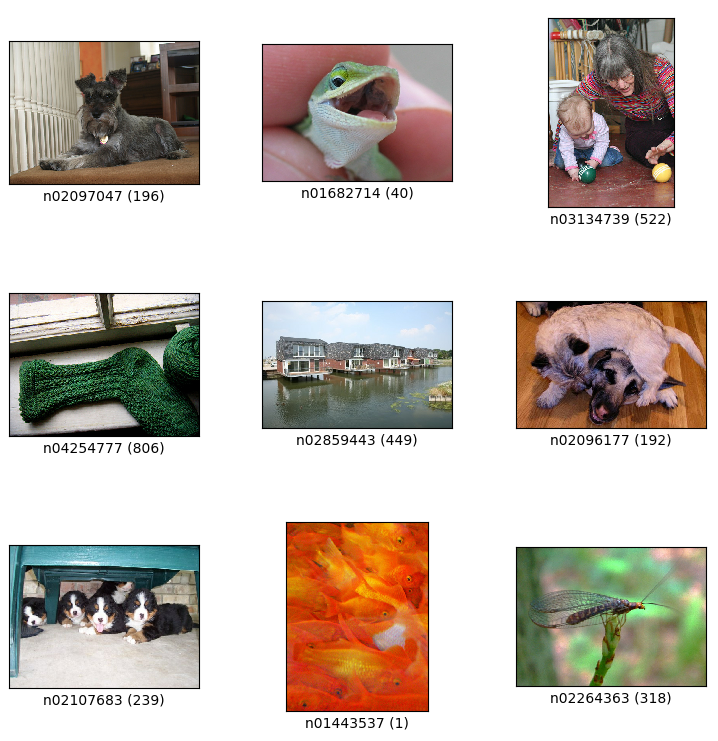
\includegraphics[width=0.7\linewidth]{imagenet2012-1}
	\caption{نمونه تصاویر از مجموعه‌داده
		ImageNet
		نسخه سال ۲۰۱۲ به همراه یک کلمه برای توصیف هر تصویر و نام هر فایل در داخل پرانتز}
	\label{fig:imagenet2012-1}
\end{figure}


\section{روش های مبتنی بر کانولوشن}

Pathak
و همکاران در \cite{pathakContextEncodersFeature2016}
یک الگوریتم یادگیری ویژگی‌های بصری بدون نظارت \LTRfootnote{Unsupervised} ارائه داده‌اند که بر اساس پیش‌بینی پیکسل مبتنی بر زمینه هدایت می‌شود. به‌طور مشابه با خودرمزگذارها
\LTRfootnote{Autoencoders}
، آن‌ها کدگذاران زمینه (\lr{Context Encoders}) را پیشنهاد کرده‌اند – یک شبکه عصبی کانولوشنی که برای تولید محتوای یک ناحیه دلخواه از تصویر، با توجه به محیط اطراف آن آموزش داده شده است. برای موفقیت در این وظیفه، معماری پیشنهادی باید هم محتوای کل تصویر را درک کنند و هم فرضیه‌ای معقول برای قسمت‌های حذف‌شده ارائه دهند.  

آن‌ها در فرایند آموزش کدگذار زمینه، از دو رویکرد استفاده کرده‌اند: یکی اتکای صرف به تابع هزینه بازسازی پیکسل-محور استاندارد بر اساس نرم دوم (\lr{L2 Loss})، و دیگری ترکیب بازسازی با یک تابع هزینه رقابتی (\lr{Adversarial Loss}) پیشنهاد شده در شبکه های GAN
\cite{goodfellowGenerativeAdversarialNetworks2014}.
نتایج نشان داده است که رویکرد دوم خروجی‌هایی با وضوح بالاتر تولید می‌کند، زیرا بهتر می‌تواند حالت‌های چندگانه در خروجی را مدیریت کند. "حالت‌های چندگانه" به این معناست که برای یک ناحیه گمشده در تصویر، چندین امکان معنایی و بصری معتبر برای پر کردن آن وجود دارد. به عبارت دیگر، ناحیه گمشده می‌تواند به‌طور همزمان با محتوای مختلفی که همگی با زمینه تصویر سازگار هستند، پر شود. این موضوع به دلیل تعدد راه‌حل‌های ممکن در مسئله ترمیم تصویر رخ می‌دهد.\\


\begin{table}[h!]
	\centering
	\begin{tabular}{|c|c|c|c|}
		\hline
		\textbf{روش} & \textbf{\lr{L1} میانگین} & \textbf{\lr{L2} میانگین} & \textbf{\lr{PSNR} (بالاتر بهتر)} \\ \hline
		\lr{NN-inpainting (HOG)} \cite{haysSceneCompletionUsing2007} & \lr{19.92\%} & \lr{6.92\%} & \lr{12.79 dB} \\ \hline
		\lr{NN-inpainting} (بردار ویژگی‌های کدگذار زمینه) & \lr{15.10\%} & \lr{4.30\%} & \lr{14.70 dB} \\ \hline
		کدگذار زمینه (ترکیبی) & \lr{09.37\%} & \lr{1.96\%} & \lr{18.58 dB} \\ \hline
	\end{tabular}
	\caption{مقایسه روش‌ کدگذار زمینه با روش های دیگر بر اساس \lr{L1} میانگین، \lr{L2} میانگین و \lr{PSNR} روی مجموعه‌داده خیابان های پاریس.}
	\label{tab:context_encoders_inpainting_results}
\end{table}


\begin{figure}
	\centering
	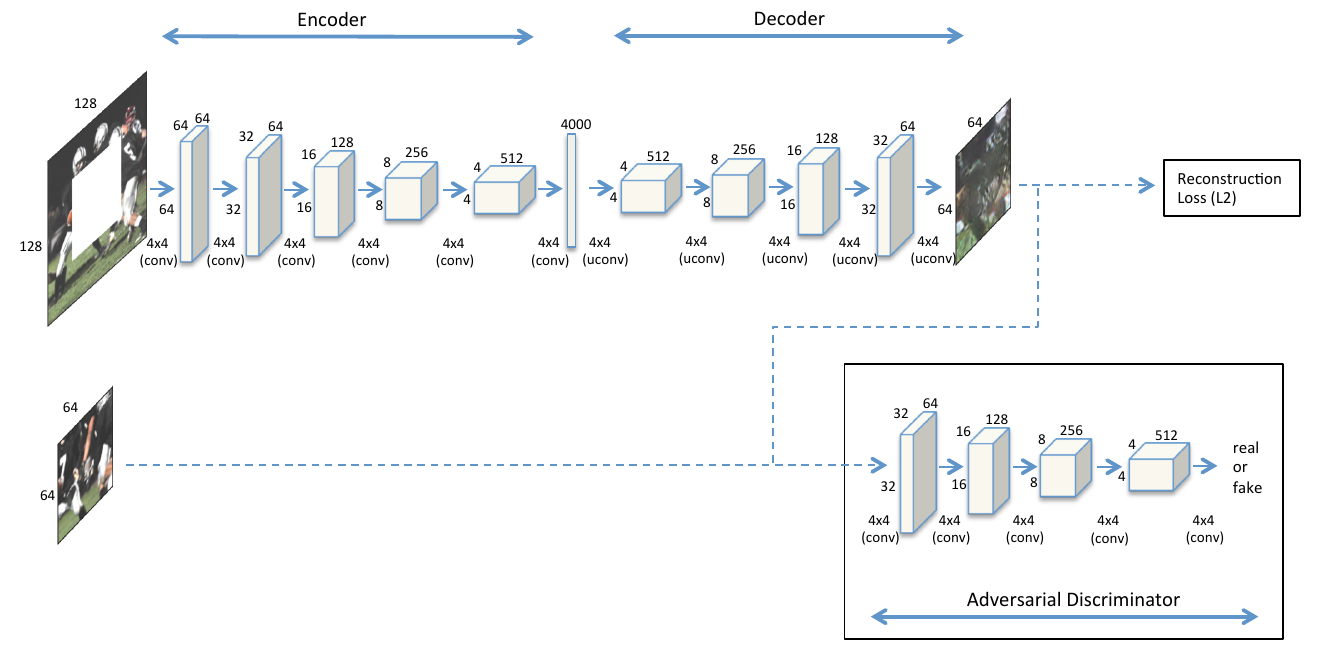
\includegraphics[width=1\linewidth]{pathakGanArch}
	\caption{معماری کدگذار زمینه که با ترکیب توابع هزینه بازسازی و رقابتی برای ترمیم معنایی آموزش دیده است.}
	\label{fig:pathakganarch}
\end{figure}



\begin{figure}
	\centering
	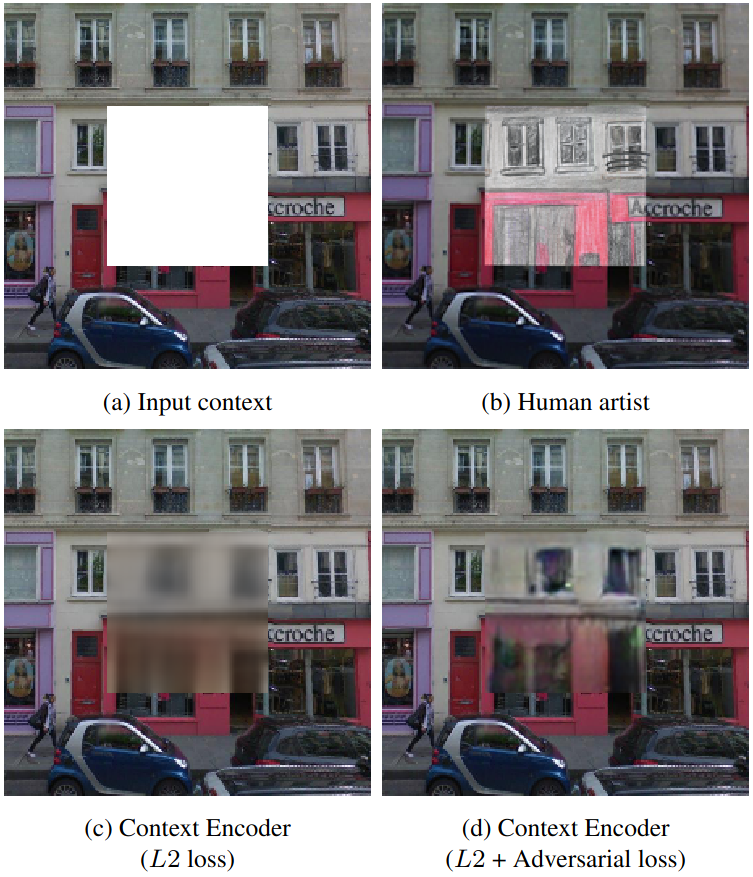
\includegraphics[width=0.7\linewidth]{figs/contextencodersLossComparison}
	\caption{مقایسه کیفی  استفاده از تابع هزینه نرم  ۲ در مقابل استفاده از یک تابع هزینه رقابتی در خروجی های تولید شده. 
		(a) عکس ورودی با یک قسمت از دست رفته 
		(b) یک انسان هنرمند مشکلی در ترمیم این تصویر ندارد 
		(c)
ترمیم خودکار تصویر با استفاده از کدگذار زمینه که توسط تابع هزینه بازسازی بر اساس نرم ۲ آموزش داده شده است.
	(d)
ترمیم خودکار تصویر با استفاده از کدگذار زمینه که توسط تابع هزینه رقابتی آموزش داده شده است.
}
	\label{fig:contextencoderslosscomparison}
\end{figure}



آن‌ها دریافتند  کدگذارهای زمینه بازنمایی هایی یاد می‌گیرند که نه‌تنها ظاهر، بلکه معنای ساختارهای بصری را نیز در بر می‌گیرد. اثربخشی این ویژگی‌های یادگرفته‌شده به‌طور کمّی برای پیش‌آموزش شبکه‌های عصبی کانولوشنی در وظایف طبقه‌بندی، تشخیص و قطعه‌بندی نشان داده شده است. علاوه بر این، کدگذارهای زمینه می‌توانند برای وظایف ترمیم معنایی تصاویر مورد استفاده قرار گیرند، چه به‌صورت مستقل و چه به‌عنوان نقطه شروع برای روش‌های غیرپارامتری.
\begin{figure}
	\centering
	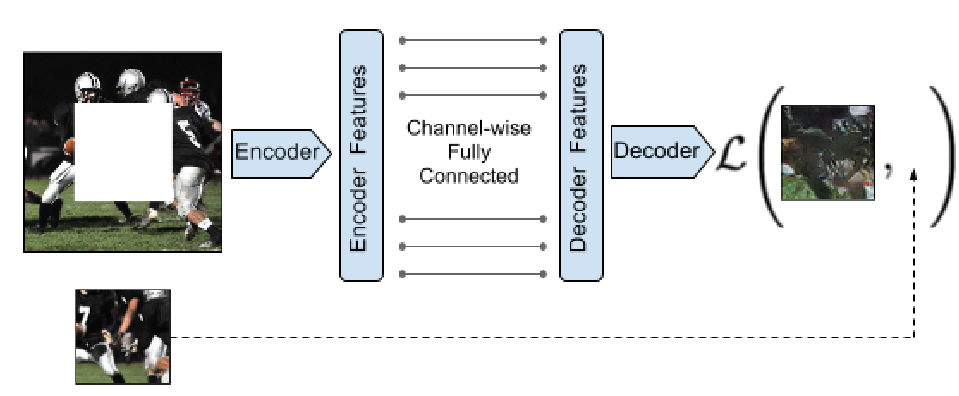
\includegraphics[width=0.7\linewidth]{figs/contextencodersArchitecture}
	\caption[معماری کلی Context Encoders]{
	تصویر زمینه از طریق بخش رمزگذار عبور داده می‌شود تا ویژگی‌هایی استخراج شوند که از طریق یک لایه کاملاً متصل کانال‌محور به رمزگشا متصل می‌شوند. سپس، رمزگشا نواحی حذف‌شده تصویر را تولید می‌کند.}
	\label{fig:contextencodersarchitecture}
\end{figure}

به دنبال این روش، روش های بسیاری بر پایه GAN ابداع شدند. 
\cite{caoLearningSketchTensor2021}
\cite{guoImageInpaintingConditional2024}
\cite{liRecurrentFeatureReasoning2020}
\cite{nazeriEdgeConnectGenerativeImage2019}
\cite{pengGeneratingDiverseStructure2021}

به عنوان مثال ایزُوکا و همکاران یک رویکرد نوین برای تکمیل تصویر ارائه دادند
\cite{iizukaGloballyLocallyConsistent2017}
که تصاویر به‌دست‌آمده هم از نظر محلی و هم از نظر سراسری سازگار بودند. با استفاده از یک شبکه عصبی کاملاً کانولوشنی، آن‌ها توانستند تصاویر با وضوح‌های دلخواه را با پر کردن نواحی گم‌شده به هر شکل تکمیل کنند. برای آموزش این شبکه تکمیل تصویر به‌طور سازگار، از متمایزکننده‌های بافت سراسری و محلی استفاده کردند که به‌طور خاص برای تشخیص تصاویر واقعی از تصاویر تکمیل‌شده آموزش دیده‌اند. متمایزکننده سراسری کل تصویر را بررسی می‌کند تا ارزیابی کند که آیا تصویر به‌طور کلی هماهنگ است یا نه، در حالی که متمایزکننده محلی فقط ناحیه‌ای کوچک متمرکز بر ناحیه تکمیل‌شده را بررسی می‌کند تا از سازگاری محلی وصله‌های تولیدشده اطمینان حاصل کند. سپس شبکه تکمیل تصویر برای فریب دادن هر دو شبکه متمایزکننده بافت آموزش داده می‌شود، که نیاز به تولید تصاویری دارد که از نظر سازگاری کلی و جزئیات با تصاویر واقعی غیرقابل تمایز باشند. این رویکرد نشان داد که می‌تواند برای تکمیل طیف وسیعی از صحنه‌ها استفاده شود. علاوه بر این، در مقایسه با رویکردهای مبتنی بر وصله مانند \lr{PatchMatch}، رویکرد آن‌ها می‌تواند تکه‌هایی تولید کند که در جای دیگری از تصویر ظاهر نمی‌شوند، که این امکان را می‌دهد که تصاویر اشیاء با ساختارهای آشنا و بسیار خاص، مانند صورت‌ها، به‌طور طبیعی تکمیل شوند.\\

\begin{table}[ht]
	\centering
	\begin{tabular}{|c|c|c|c|}
		\hline
		\textbf{} & \textbf{مبتنی بر وصله} & \textbf{کدگذار زمینه} & \textbf{ایزوکا و همکاران} \\
		\hline
		\textbf{اندازه تصویر} & \textbf{هر اندازه} & ثابت & \textbf{هر اندازه} \\
		\hline
		\textbf{سازگاری محلی} & \textbf{بله} & خیر & \textbf{بله} \\
		\hline
		\textbf{معناشناسی} & خیر & \textbf{بله} & \textbf{بله} \\
		\hline
		\textbf{اشیاء نوین} & خیر & \textbf{بله} & \textbf{بله} \\
		\hline
	\end{tabular}
	\caption{مقایسه روش‌ ارائه شده توسط ایزوکا  و همکاران در مقایسه با کدگذارهای زمینه و روش های الگوریتمی مبتنی بر وصله.}
\end{table}


\begin{figure}
	\centering
	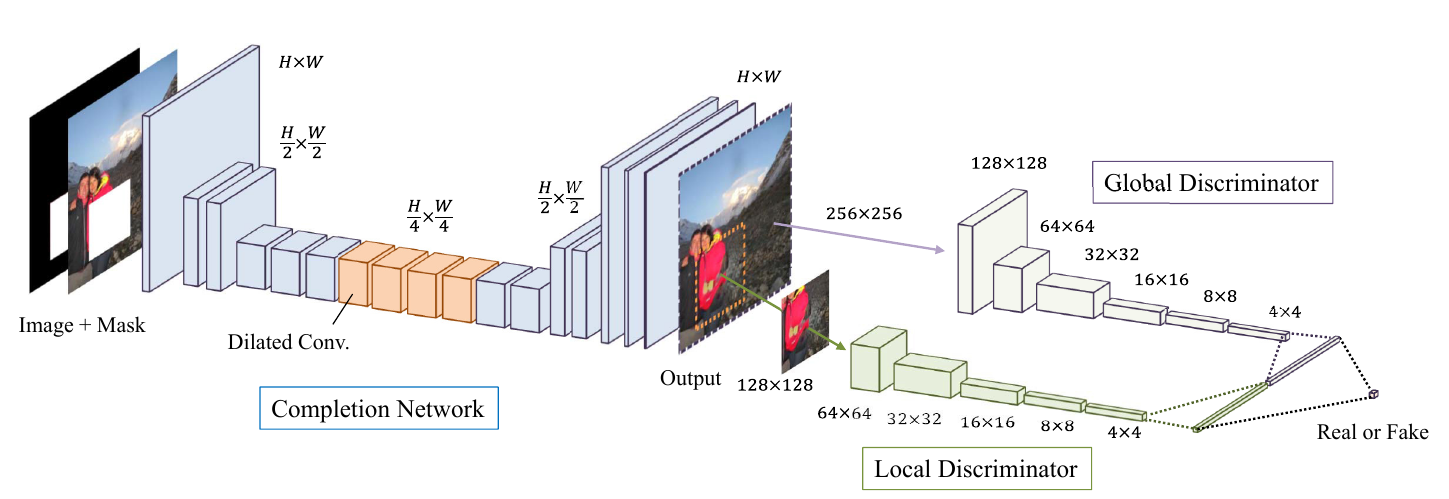
\includegraphics[width=1\linewidth]{IISUKAArch1}
	\caption{مروری بر معماری ایزوکا و همکاران برای یادگیری ترمیم تصویر. این معماری شامل یک شبکه تکمیل و دو شبکه متمایزکننده کمکی زمینه است که تنها برای آموزش شبکه تکمیل  کننده استفاده می‌شوند و در طول آزمایش (\lr{Inference})
		 مورد استفاده قرار نمی‌گیرند. شبکه متمایزکننده سراسری کل تصویر را به‌عنوان ورودی می‌گیرد، در حالی که شبکه متمایزکننده محلی تنها ناحیه‌ای کوچک اطراف ناحیه تکمیل‌شده را به‌عنوان ورودی می‌گیرد. هر دو شبکه متمایزکننده آموزش داده می‌شوند تا تشخیص دهند که آیا تصویر واقعی است یا توسط شبکه تکمیل‌کننده ساخته شده است، در حالی که شبکه تکمیل‌کننده برای فریب دادن هر دو شبکه متمایزکننده آموزش داده می‌شود.}
	\label{fig:iisukaarch1}
\end{figure}


\begin{figure}
	\centering
	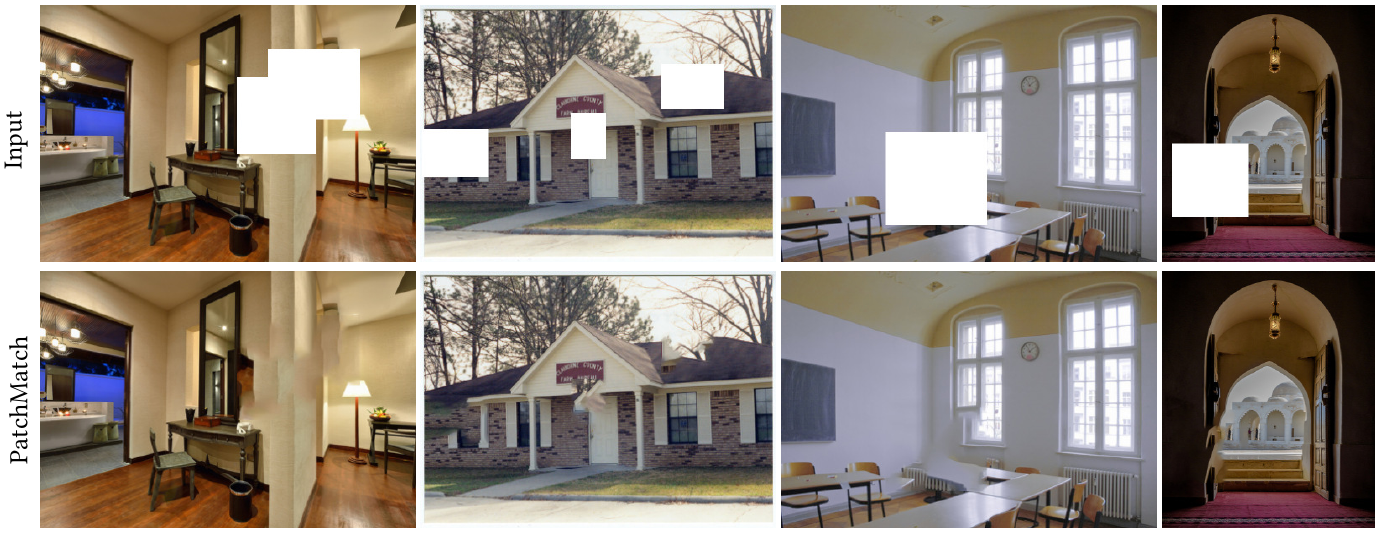
\includegraphics[width=1\linewidth]{IISUKqual1}
	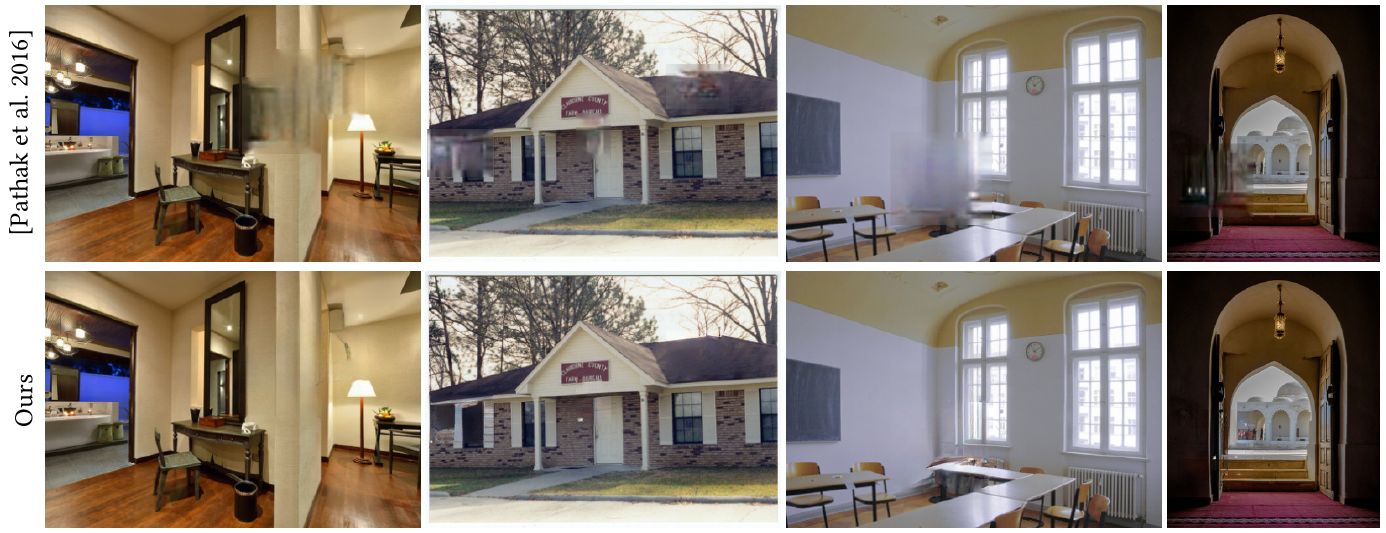
\includegraphics[width=1\linewidth]{IISUKqual2}
	\caption{نتایج کیفی مدل ایزوکا و همکاران در مقایسه با دو روش بیان شده  قبلی بر روی مجموعه‌داده \lr{Places2}}
	\label{fig:iisukqual2}
\end{figure}


\begin{figure}
	\centering
	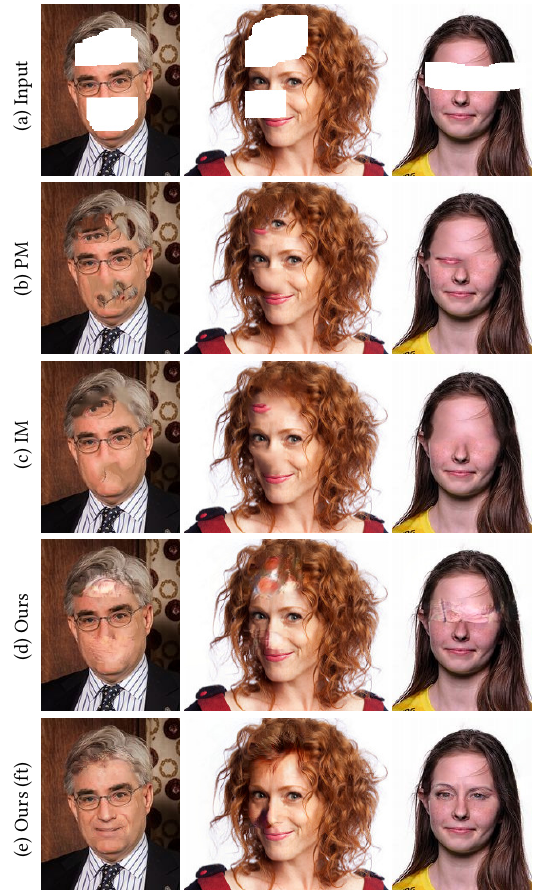
\includegraphics[width=0.5\linewidth]{IISUKqual3}
	\caption{نتایج کیفی مدل ایزوکا و همکاران در مقایسه با دو روش بیان شده  و در مقایسه با معماری ایزوکا، فاین‌تیون شده برای تصاویر چهره. توانایی ساخت ویژگی های نوین چهره در مدل فاین‌تیون شده (FT) مشهود است.}
	\label{fig:iisukqual3}
\end{figure}


\begin{figure}
	\centering
	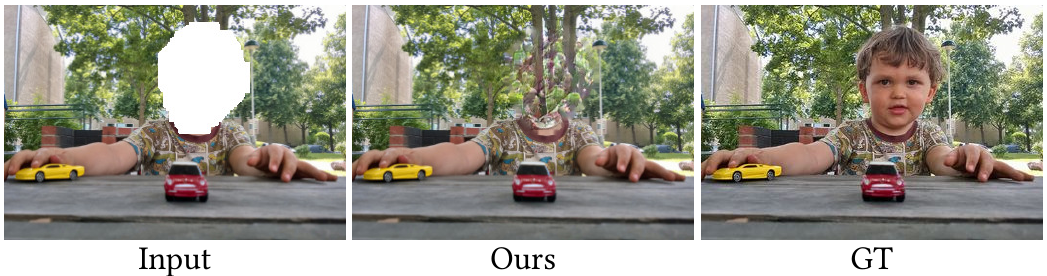
\includegraphics[width=1\linewidth]{IISUKfail}
	\caption{نمونه ای از ترمیم شکست‌خورده توسط معماری ایزوکا و همکاران. مدل آنها نتوانست اشیاء با ساختار بسیار پیچیده را ترمیم کند.}
	\label{fig:iisukfail}
\end{figure}


\warningToSelfExpandable

این استراتژی‌ها همگی به دنبال این هستند که روش‌های مؤثری برای استخراج اطلاعات معتبر از نواحی شناخته‌شده تصویر به منظور پر کردن حفره‌ها پیدا کنند. هدف اصلی این رویکردها، بهره‌برداری بهینه از اطلاعات زمینه‌ای و استفاده از آن‌ها برای بازسازی نواحی گمشده است. با این حال، این روش‌ها هنوز با مشکلی اساسی روبرو هستند: از دست رفتن اطلاعاتی که در فرآیند نمونه‌برداری رو به پایین (\lr{Downsampling}) در شبکه‌های کانولوشنی رخ می‌دهد.  

این فرآیند نمونه‌برداری که برای کاهش ابعاد داده و افزایش بازده محاسباتی در شبکه‌های عصبی مورد استفاده قرار می‌گیرد، اغلب منجر به حذف جزئیات ظریف و اطلاعات ضروری می‌شود که می‌توانند برای بازسازی دقیق‌تر و واقعی‌تر مناطق گمشده نقش کلیدی ایفا کنند. بنابراین، یکی از چالش‌های مهم این است که چگونه می‌توان ضمن بهره‌گیری از مزایای نمونه‌برداری رو به پایین، تأثیرات منفی آن را کاهش داد و اطلاعات از دست رفته را تا حد ممکن حفظ کرد.






